\newpage
%********************************************************************************
\section{FEBA Reflood Separate Effect Test Facility}\label{sec:reflood_feba_setf}
%********************************************************************************

% Introductory paragraph
A series of \gls[hyper=false]{feba} experiments was conducted in the 1980s at the Karlsruhe Institute of Technology (KIT)\footnote{formerly Kernforschungzentrum Karlsruhe (KfK)}
to improve the knowledge of the \gls[hyper=false]{ht} mechanism during reflooding,
taking into account the effects of spacer grids and flow blockage due to fuel rod ballooning.
The data from the facility was also intended to validate the \gls[hyper=false]{th} models and codes available at the time.

% FEBA Facility
The facility consisted of a test section with full height $5 \times 5$ bundle of \textsc{PWR} fuel rod simulator (Fig.~\ref{fig:feba_setf}a) enclosed in a rectangular stainless steel housing (Fig.~\ref{fig:feba_setf}b).
An approximate cosine power profile was mapped over of the height of the fuel rod simulators (Fig.~\ref{fig:feba_setf}c).
Seven spacer grids were used to provide mechanical support of the fuel rod simulators (Fig.~\ref{fig:feba_setf}d).

\begin{figure}[bth]
	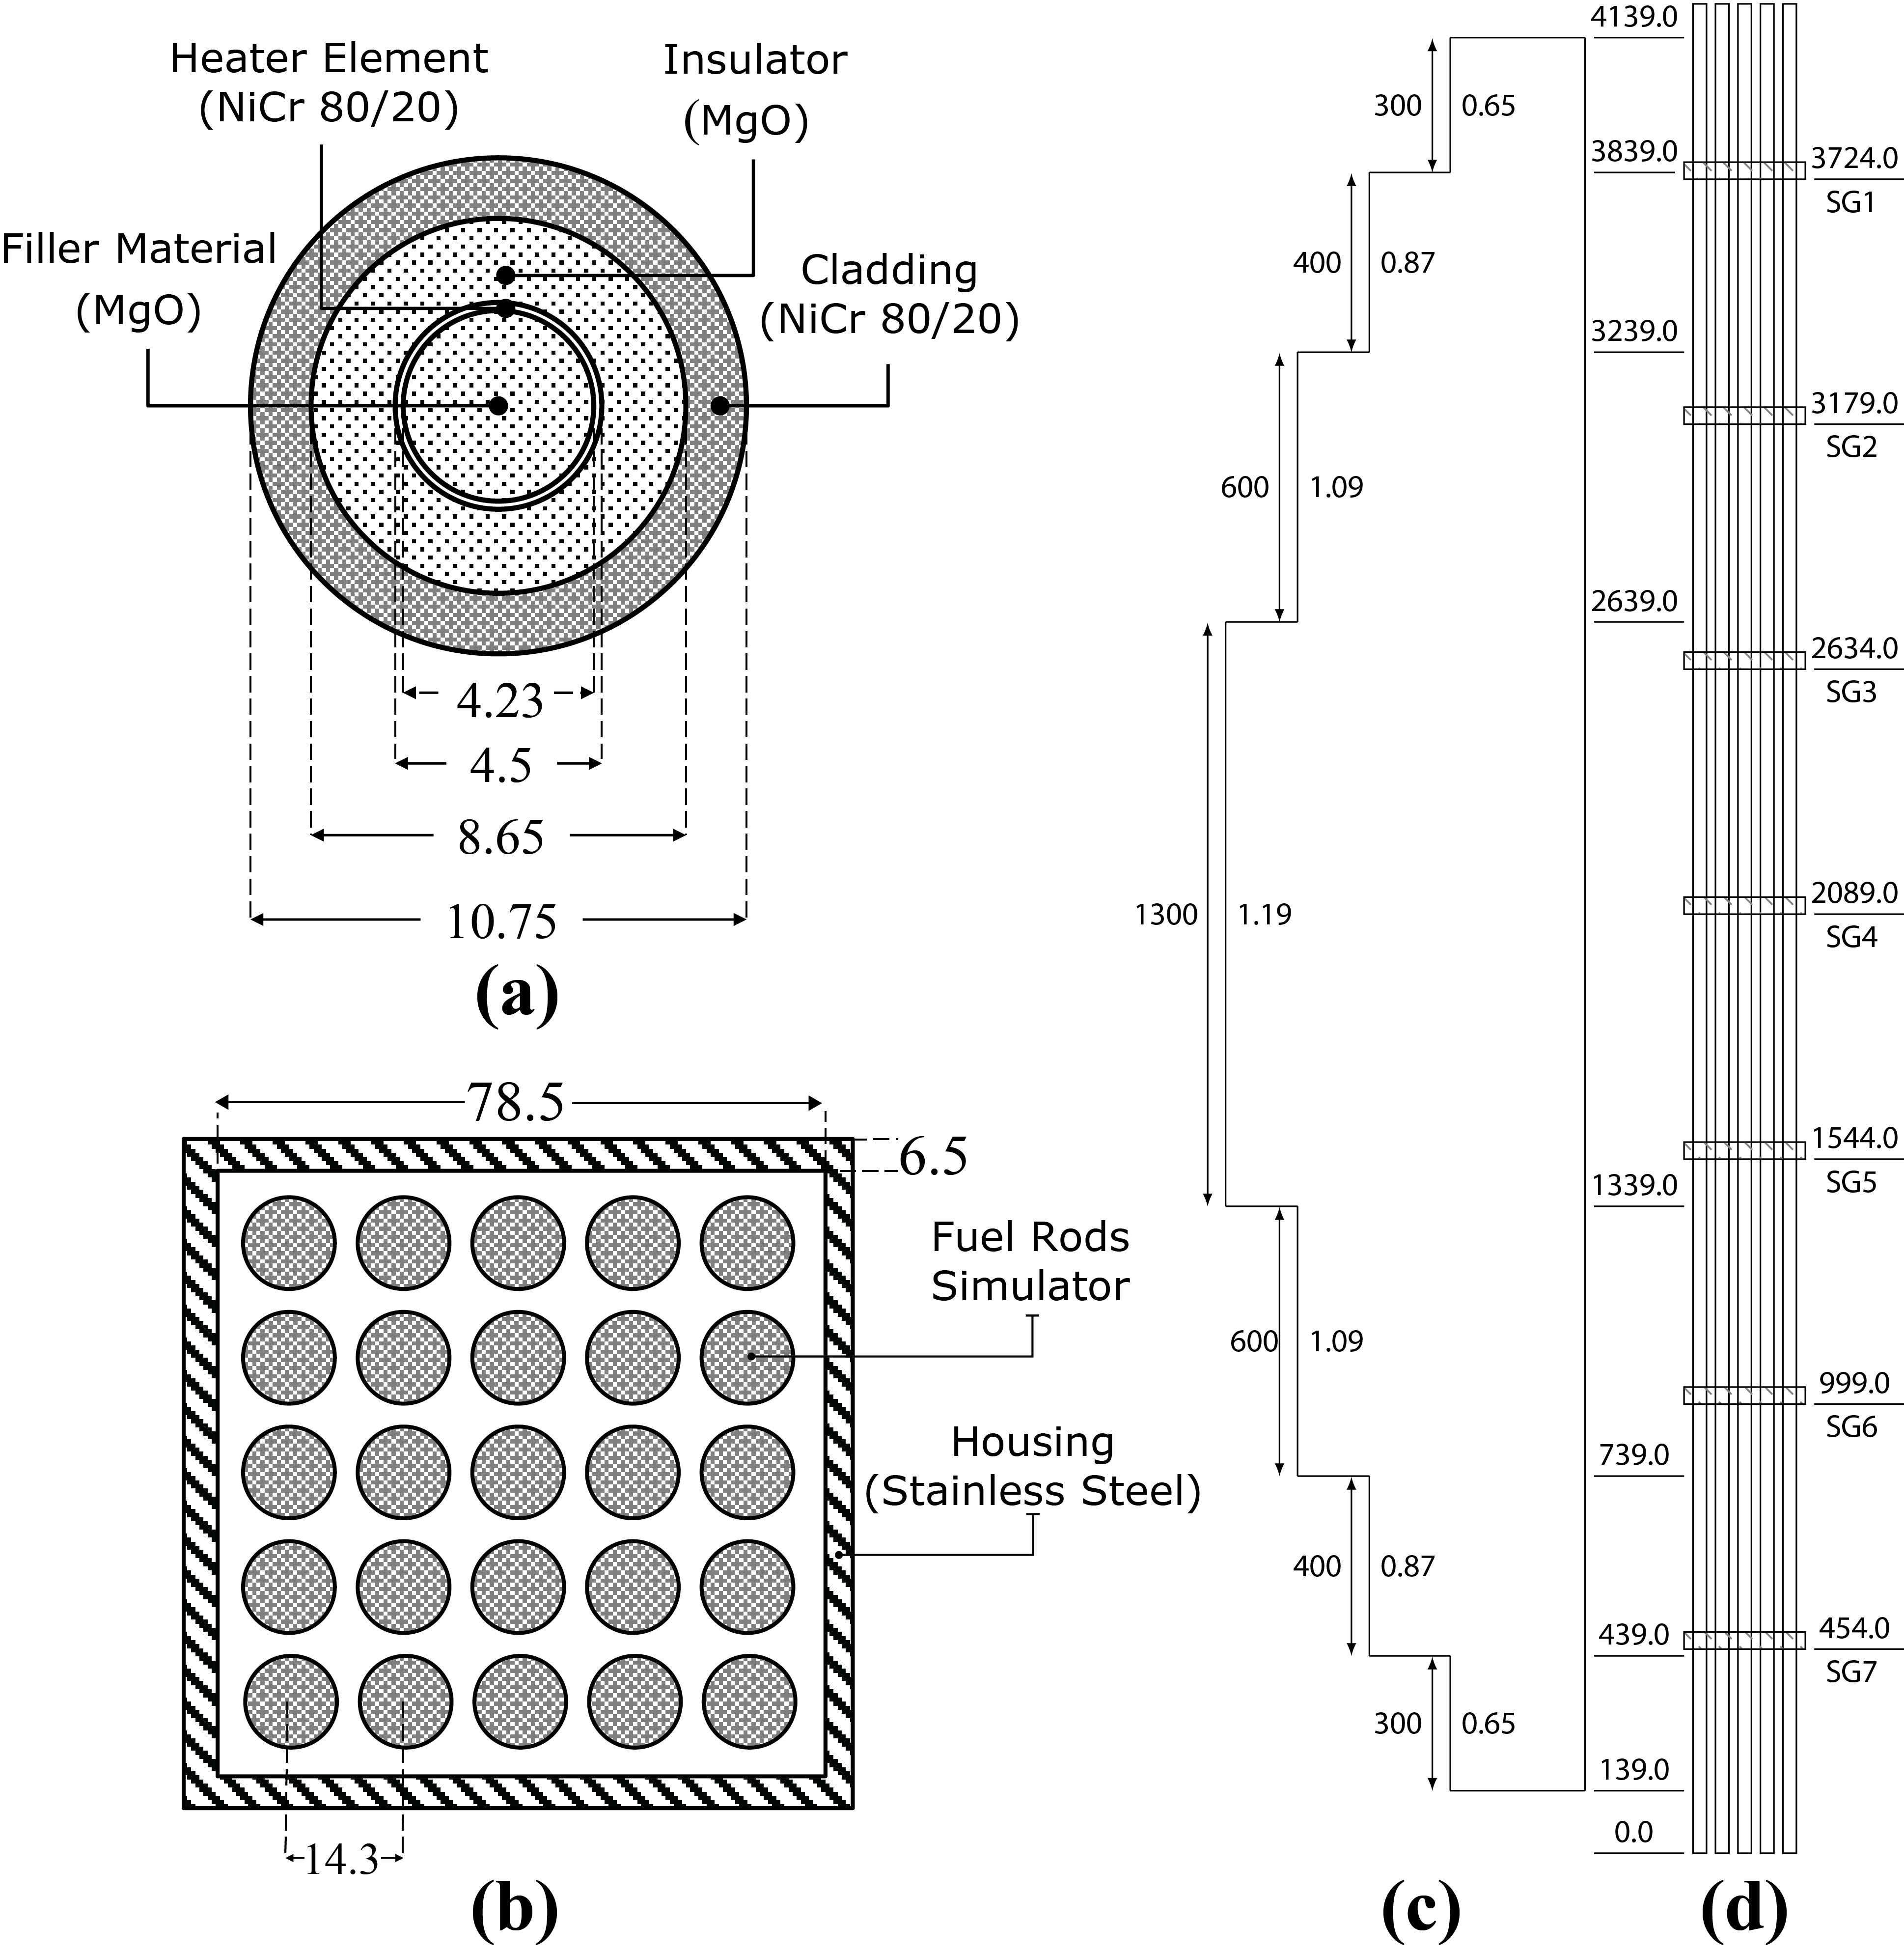
\includegraphics[width=1.0\textwidth]{../figures/chapter2/febaTestSection/febaTestSection.png}
	\caption[FEBA experimental facility.]{(a) The cross section of the fuel rod simulators used in \gls[hyper=false]{feba} separate-effect test facility. (b) the cross section of the test section including the rectangular housing. (c)  The approximate cosine power profile, numbers written inside the bix are the relative power $P/P_{avg}$. (d) The location of spacer grids in the test section. All dimensions are in units of milimeters $[mm]$.}\label{fig:feba_setf}
\end{figure}

% How the experiment was conducted
During the initialization phase of the experiment,
the test section was heated up at low nominal power ($200 \ [kW]$) to achieve a specified initial heater rod temperature, with no liquid present in the test section.
The transient phase of the experiment was initiated by ramping up the power according to $120$\% (ANS\footnote{American National Standard}) decay heat power curve while simultaneously injecting subcooled liquid from the bottom of the test section.
Several temperature measurements at the outer surface of the heater rods, hereinafter referred to as the clad temperature, were taken at different axial locations during the course of each transient test.

% FEBA Test Series
Eight different test series were performed in the FEBA facility. 
The first two test series (I and II) used two different numbers of spacer grids, seven and six, respectively.
The middle spacer grid was removed in test series II to investigate the effect of spacer grids in a reflood transient.
The other test series used different flow area blockage sizes at midheight of the test section to investigate the effect of rod ballooning of different sizes.
In each test series, combinations of two different inlet liquid velocities and three different system backpressure were imposed.

% FEBA Test Series I
The present thesis analyzed only the experimental data sets from the test series I.
This particular test run was used as the base experimental setup with all seven spacer grids mounted and no flow area blockage.
Different experimental runs corresponding to different experimental conditions of test series I are given in Table~\ref{tab:feba_exp}.

\begin{table}[h]
	\myfloatalign
	\caption[FEBA test series I experimental conditions]{\gls[hyper=false]{feba} test series I experimental conditions.}
	\label{tab:feba_exp}
	\begin{tabularx}{\textwidth}{cccc} \toprule
		Test No. & System Pressure & Flooding Rate  			& Duration of Test\\ 
		         & $[bar]$         & $[cm \cdot s^{-1}]$ 	& $[s]$						\\ \midrule
		$216$ & $4.12$  & $3.81$ & $600$\\
		$214$ & $4.11$  & $5.77$ & $400$\\
		$223$ & $2.21$  & $3.82$ & $900$\\
		$218$ & $2.08$  & $5.81$ & $550$\\
		$220$ & $6.18$  & $3.85$ & $400$\\
		$222$ & $6.18$  & $5.78$ & $300$\\
		\bottomrule
	\end{tabularx}
\end{table}

% Experimental data in the FEBA
Three types of times series measurement were recorded in the experiment.
These included thermocouple to measure the clad temperature (referred to as $TC$) at $8$ different axial locations,
pressure probe to measure the pressure drop (referred to as $DP$) at $4$ different axial segments of the test assembly,
and a collecting tank measuring the mass of water carried over at the end of the test section (i.e., the liquid carryover, referred to as $CO$).
The axial locations of the thermocouples and the axial segments at which the pressure drop were measured are summarized in Table~\ref{tab:feba_exp_data}. 
Note that the thermocouple ID was inverted, the increasing number indicated a decreasing elevation, that is, $TC1$ at the top and $TC8$ at the bottom of the assembly.
\begin{table}[h]
	\myfloatalign
	\caption[Locations of the thermocouples and the pressure drop measurements from the FEBA experiment.]{Locations of the thermocouples and the pressure drop measurements from the FEBA experiment.}
	\label{tab:feba_exp_data}
	\begin{tabularx}{\textwidth}{ccc} \toprule
		Types of  	& ID & Axial Locations (or segments) \\ 
		Measurement &    & $[m]$ \\ \midrule
		\multirow{8}{*}{$TC$} & $TC1$  	& $4.1$ \\
		                      & $TC2$  	& $3.6$ \\
	                        & $TC3$  	& $3.0$ \\
		                      & $TC4$  	& $2.4$ \\
		                      & $TC5$  	& $1.9$ \\
		                      & $TC6$  	& $1.3$ \\
													& $TC7$  	& $0.8$ \\
													& $TC8$  	& $0.3$ \\
		\midrule
		\multirow{4}{*}{$DP$} & Bottom  & $0.0 - 1.7$ \\
		                      & Middle  & $1.7 - 2.5$ \\
	                        & Top  		& $2.3 - 4.1$ \\
		                      & Total 	& $0.0 - 4.1$ \\
		\bottomrule
	\end{tabularx}
\end{table}

% Source of FEBA Information
The facility specification and the test data are compiled in a series of reports that are available at the KIT library website.
The specifications and the data provide a valuable source of information for \gls[hyper=false]{trace} code assessment since the \gls[hyper=false]{feba} experiment is not part of the original validation matrix of the code. 
More details can be found in \cite{Ihle1984}.